\documentclass[12pt,letterpaper,twocolumn]{article}
\usepackage[utf8]{inputenc}
\usepackage[margin=1in,left=0.7in,right=0.7in]{geometry}
\usepackage[cmex10]{amsmath}
\usepackage{amsfonts}
\usepackage{amssymb}
\usepackage{float}
\usepackage{enumerate}
\usepackage[none]{hyphenat}
\usepackage{graphicx}
\usepackage{parskip}
\setlength{\parindent}{0cm}
\pagenumbering{gobble}

\addtolength{\topmargin}{-1.0cm}

\title{\textbf{AI1110 Assignment 1(Paper 2018)}}
\author{\textbf{Dasari Srinith (cs21btech11015)}}
\date{}

\begin{document}

\maketitle

\section*{Q4 (c)}
    Solve $x^2 + 7x = 7$ and give your answer correct to two decimals.
\vspace{-0.5cm}
\section*{Solution}

    Given,
    To Find the roots of
    \begin{align}
        x^2 +7x -7 = 0
    \end{align}
    We know that for the quadratic equation of form
    \begin{align}
        ax^2 + bx +c = 0
    \end{align}
    the roots are
    \begin{align}
        \dfrac{-b+\sqrt{b^2 -4ac}}{2a}&,\dfrac{-b-\sqrt{b^2 -4ac}}{2a}\\[10pt]
        \implies \dfrac{-7+\sqrt{49-4(-7)}}{2(1)}&,
        \dfrac{-7-\sqrt{49 -4(-7)}}{2(1)}\\[10pt]
        \implies \dfrac{-7+\sqrt{77}}{2}&,
        \dfrac{-7-\sqrt{77}}{2}\\[10pt]
        \implies \dfrac{-7+8.7749}{2} &,\dfrac{-7-8.7749}{2}\\[10pt]
        \implies -7.8874 &, 0.8874
    \end{align}
($\sqrt{77}$ can be found by long division method up to four decimals)
    
$\implies$ The roots are -7.8874, 0.8874
    
On rounding them off to 2 decimal places we get the roots as -7.89 and 0.89.
    
\begin{figure}[H]
    \centering
    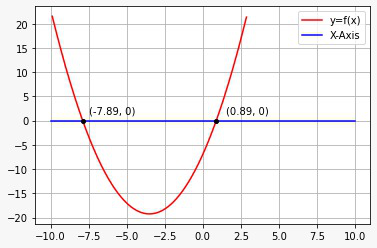
\includegraphics[width=8cm]{_plot.png}
    \caption{Plot of the quadratic equation}
\end{figure}
 
$\therefore$ The solutions of 
\begin{align}
    x^2 + 7x = 7
\end{align}
are
\begin{align}
    x &= -7.89\\
    x &= 0.89
\end{align}
    
\end{document}
